\subsection{Accuracy}
\label{sec:hash-accuracy}
Assessing the accuracy of file hash feeds presents a problem: there is no
universal ground truth to determine if a file is malicious or benign. Thus,
to gauge the accuracy of the feeds, I use two metrics: a check for malicious
hashes against VirusTotal, and a check for benign hashes against Shadowserver's
Bin Check service. Note that all the percentages discussed below are based on
the \textit{Volume} of each feed.

\subsubsection{VirusTotal}

VirusTotal is a service that is often used when analyzing
malware to get a base of information about a suspected file.
Anyone can upload a file to be scanned. Upon submission, these files will be
scanned by more than 70 antivirus scanners, which creates a report on how many
antivirus scanners mark it malicious, among other information. In this analysis,
I query VirusTotal for the hashes in each file hash feed and then inspect the
percent of hashes that are marked as malicious and how many AV scanners have
recorded them. Due to the high volume of the FB Malware feed and the query
rate limit of VirusTotal, I randomly sampled 80,000 hashes from the feed for
this analysis.

Table~\ref{tab:md5-volume-2} shows a breakdown of the base detection rates 
for
each feed from VirusTotal. As the PA feeds decrease in volume, the rates at
which they are found in VirusTotal also decreases. The larger PA feeds have a
much higher detection rate than their smaller counterparts. On the other hand,
FB Malware only has 37\% of its data detected by antivirus scanners and 50\% in
VirusTotal with no detection despite being the largest feed. This could indicate
that FB Malware focuses on threats that specifically target Facebook and that
are not as relevant to most VirusTotal users, such as malicious browser
extensions~\cite{dekoven2017malicious, jagpal2015trends, kapravelos2014hulk}.
This might undermine the limited coverage of VirusTotal as an oracle to detect
targeted threats that are not of broader interest.

\begin{figure}[t]
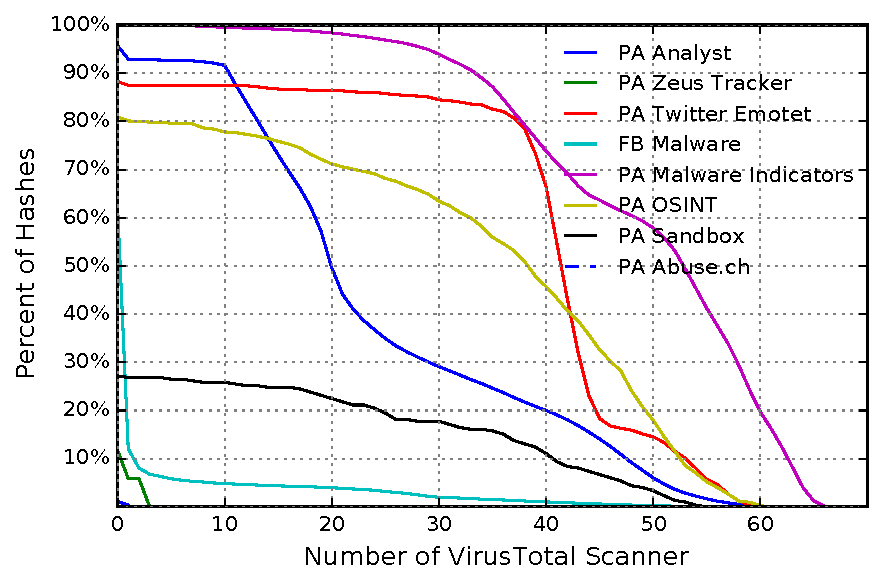
\includegraphics[width=0.8\columnwidth]{data_character/images/hash_vt_cdf.pdf}
\caption{VirusTotal detection distribution.}
\label{fig:vt-cdf}
\end{figure}

To further understand how the scanners in VirusTotal report the feed's data,
I plot a graph of what percentage of hashes in each feed are detected by how many
VirusTotal scanners. As seen in Figure~\ref{fig:vt-cdf}, each point means the proportion of indicators (Y value) in a feed that is detected by \textit{over} X number of AV scanners in VirusTotal. Four feeds have more
than 50\% of their samples detected by over 20 scanners. PA Malware Indicators
and PA Twitter Emotet did not experience a large detection drop before 35 scanners,
indicating that most indicators in the two feeds are popular malicious files
recognized by many AV vendors. While PA Sandbox has a large percent of its hashes
not presented in VirusTotal, over 70\% of its samples that are detected are marked
by over 20 AV scanners, showcasing a high confidence detection.

\subsubsection{Shadowserver}

To more fully gauge the accuracy of the file hash feeds,
I also examined how each feed measured against Shadowserver's Bin Check
Service~\cite{shadowserver}. The service checks file hashes against NIST's
National Software Registry List (NSRL) in addition to Shadowserver's own repository of
known software. Table~\ref{tab:md5-volume-2} details how each feed compares with
Shadowserver's Bin Check service.

It might be expected that there would be no hash found with Shadowserver's Bin
Check service, but it is not the case. Some of the samples from the feeds that
appear in Shadowserver are well known binaries such as versions of Microsoft
Office products, Window's Service Packs, calc.exe, etc. In the event malware
injects itself into a running process, it remains plausible that some of these
well-known binaries find their way into \ti\ feeds from users wrongly attributing
maliciousness. While FB Malware has over one thousand hashes in Shadowserver, this
is not a widespread issue, as all feeds have <1\% of their hashes contained within
Shadowserver's Bin Check service.
%, shown in Table \ref{tab:md5-volume}.
This showcases that while there are a few exceptions, the feeds mostly do not
contain well-known, benign files.

\finding\ Each PA feed has a negligible rate of occurrence within Shadowserver
regardless of their VirusTotal detection, showing they do not contain generic
false positives. Larger feeds exhibit high VirusTotal detection rates except
for FB Malware, while small feeds have relatively low detection rates.
This suggests that small hash feeds might focus more on specific malicious files
that are not widely known.
FB Malware has a low VirusTotal occurrence despite
its size and has over one thousand hashes in Shadowserver, but its overall low
percentage of hashes within Shadowserver indicates that it does not contain
many known files and might have threats not typically recognized by
VirusTotal's scanners.
